\documentclass{article}

\usepackage{preamble}
\usepackage{multicol}
\usepackage[toc,page]{appendix}

\usepackage{xcolor}
\newcommand{\yht}[1]{{\color{red}[YHT: #1]}}

\usepackage[utf8]{inputenc}
\usepackage{pifont}
\usepackage{newunicodechar}
\newunicodechar{✓}{\ding{51}}
\newunicodechar{✗}{\ding{55}}

\usepackage{tikz}
\usetikzlibrary{arrows.meta,chains,
                decorations.pathreplacing,
                decorations.pathmorphing,
                decorations.shapes,
                positioning}

\usepackage{listings}
\definecolor{mGreen}{rgb}{0,0.6,0}
\definecolor{mGray}{rgb}{0.5,0.5,0.5}
\definecolor{mPurple}{rgb}{0.58,0,0.82}
\definecolor{backgroundColour}{rgb}{0.95,0.95,0.92}

\lstdefinestyle{CStyle}{
    backgroundcolor=\color{backgroundColour},
    commentstyle=\color{mGreen},
    keywordstyle=\color{magenta},
    numberstyle=\tiny\color{mGray},
    stringstyle=\color{mPurple},
    basicstyle=\footnotesize,
    breakatwhitespace=false,
    breaklines=true,
    captionpos=b,
    keepspaces=true,
    numbers=left,
    numbersep=5pt,
    showspaces=false,
    showstringspaces=false,
    showtabs=false,
    tabsize=2,
    language=C
}

\begin{document}
\frontmatter
  \title{Pre-Meeting Report}
  \author{Y{\i}ltan Hassan Temu\c{c}in}
  \maketitle
  \tableofcontents
  \mainmatter

  \section{Implementation Details}
  \subsection{Communication Back-End}
  \begin{itemize}
    \item For this implementation, I rely on Open MPI's PML layer (i.e calls to UCX tag interface)
    \item Open MPI's Persistent MPI Partitioned implementation has a bug
          (See Appendix~\ref{app:pcomm:bug} for details)
  \end{itemize}

  \subsection{MPI\_P\textless collective\textgreater\_init()}
  As there are many collectives that are required to implemented
  for a complete library, I wanted to design a generic communication schedule.
  To faciliate this,
  the only difference between each collective is the communication graph.
  Our initialization functions are as follows:
  \begin{itemize}
    \item Create communication graph that represents the communication algorithm (i.e k-nomial, linear, etc)
    \begin{itemize}
      \item The alogrithm selection would occur at this stage
    \end{itemize}
    \item Allocate request object and add it to the message progression engine.
    \item {\color{red} Question:} Does the ranks in the collective need to be matched at this point?
    \begin{itemize}
      \item For a point-to-point implementation we can deffer this
    \end{itemize}
  \end{itemize}

  \subsection{MPI\_Start()}
  \begin{itemize}
    \item Ranks that recv, post their recives for the next round
  \end{itemize}

  \subsection{MPI\_Pready()}
  \begin{itemize}
    \item Ranks that send, send the data for their partition
  \end{itemize}

  \subsection{MPI\_Parrived()}
  \begin{itemize}
    \item Ranks that only recive:
    \begin{itemize}
      \item Checks if the flag for partition has been set, if not, then enters
            the progression engine
      \begin{itemize}
        \item Entering the message progression engine is expensive but will
              deadlock if it does not enter
      \end{itemize}
    \end{itemize}
    \item Ranks that recive and forward messages to other ranks:
    \begin{itemize}
      \item Checks if the flag for partition has been set, if not, then enters
            the progression engine
      \item If the flag is true, then it calls pready for the ranks that the
            message is being forwared to
    \end{itemize}
  \end{itemize}

  \section{Performance Results}
  Results are on Niagara (ConnectX-5), good proxy for NC1225 while we dealt with teething issues.
  \subsection{Testing Methodology}
  \begin{itemize}
    \item Each Rank has $n$ threads/partitions
    \item For each rank:
    \begin{itemize}
      \item A single thread is chosen at random $t_i \in \{t_0, \cdots, t_n\}$ from a uniform distribution
      \item Some delay $\Delta$ is applied to that thread
    \end{itemize}
    \item This results in the likeley secnario where different partitions are
          blocking on different ranks
  \end{itemize}

  \subsection{Bcast - Linear Algorithm}
  \begin{itemize}
    \item Significant performance degregation for small messages
    \item Minor to negiliable performance benefit for medium/large messages
  \end{itemize}

  \begin{figure}[h]
    \centering
    \begin{subfigure}[b]{0.44\textwidth}
      \centering
      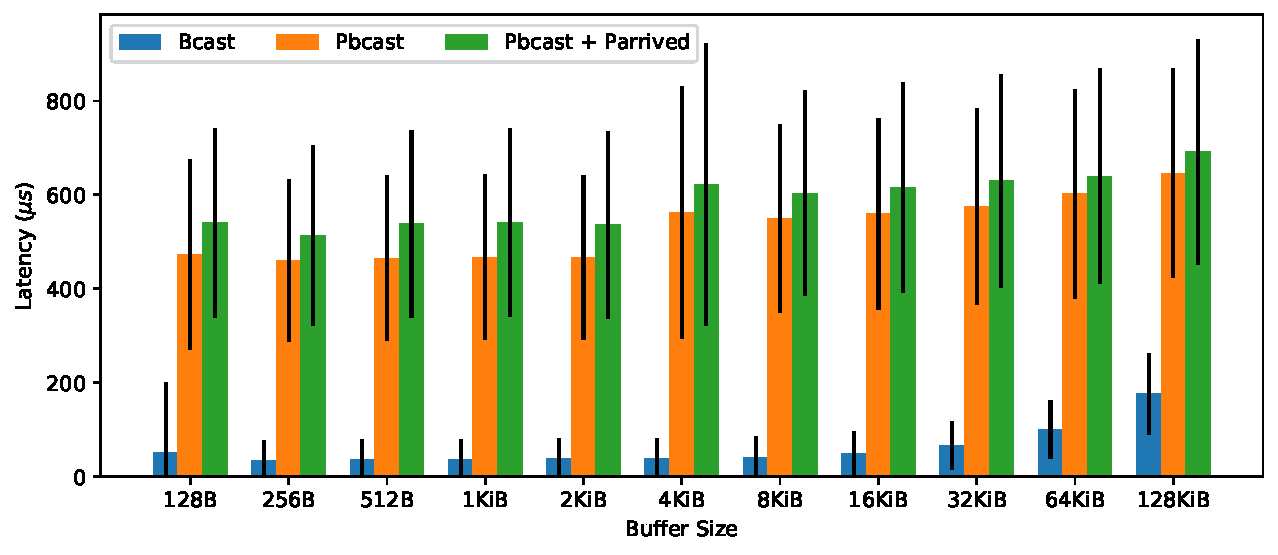
\includegraphics[width=\textwidth]{data-linear-bcast-tree/small.pdf}
      \caption{Small}
    \end{subfigure}

    \begin{subfigure}[b]{0.44\textwidth}
      \centering
      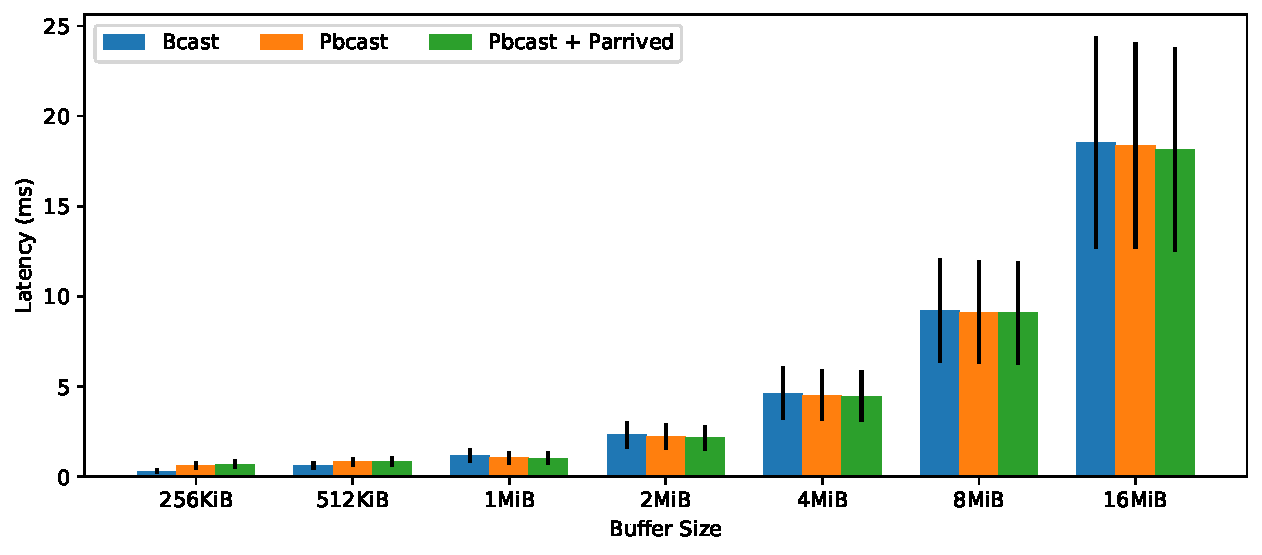
\includegraphics[width=\textwidth]{data-linear-bcast-tree/med.pdf}
      \caption{Medium}
    \end{subfigure}
    \hfill

    \begin{subfigure}[b]{0.44\textwidth}
      \centering
      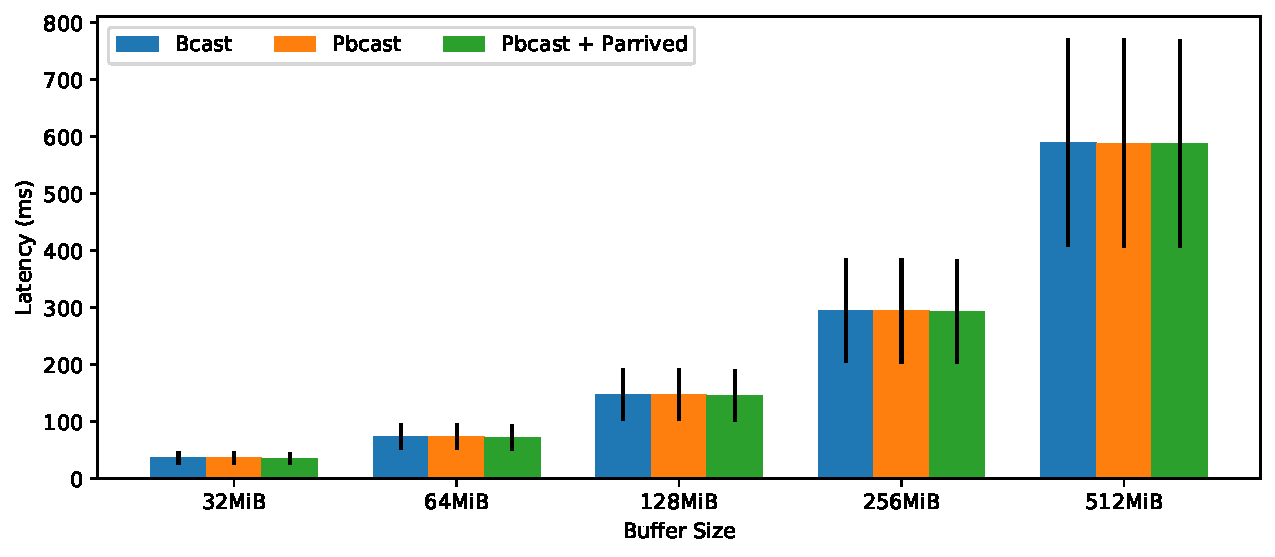
\includegraphics[width=\textwidth]{data-linear-bcast-tree/large.pdf}
      \caption{Large}
    \end{subfigure}
    \caption{Comparison of Partitioned and Traditional Broadcast communication
             pattern using the linear algorithm. Using 16 ranks with 32 threads
             (512 cores) and $\Delta = 40\mu s$.}
  \end{figure}

  \clearpage
  \subsection{Bcast - Binomial Algorithm}
  \begin{itemize}
    \item Using MPI\_Parrived has significan perfomance implications in this design
    \begin{itemize}
      \item This is the cost of entering the message progression engine
    \end{itemize}
  \end{itemize}

  \begin{figure}[h]
    \centering
    \begin{subfigure}[b]{0.44\textwidth}
      \centering
      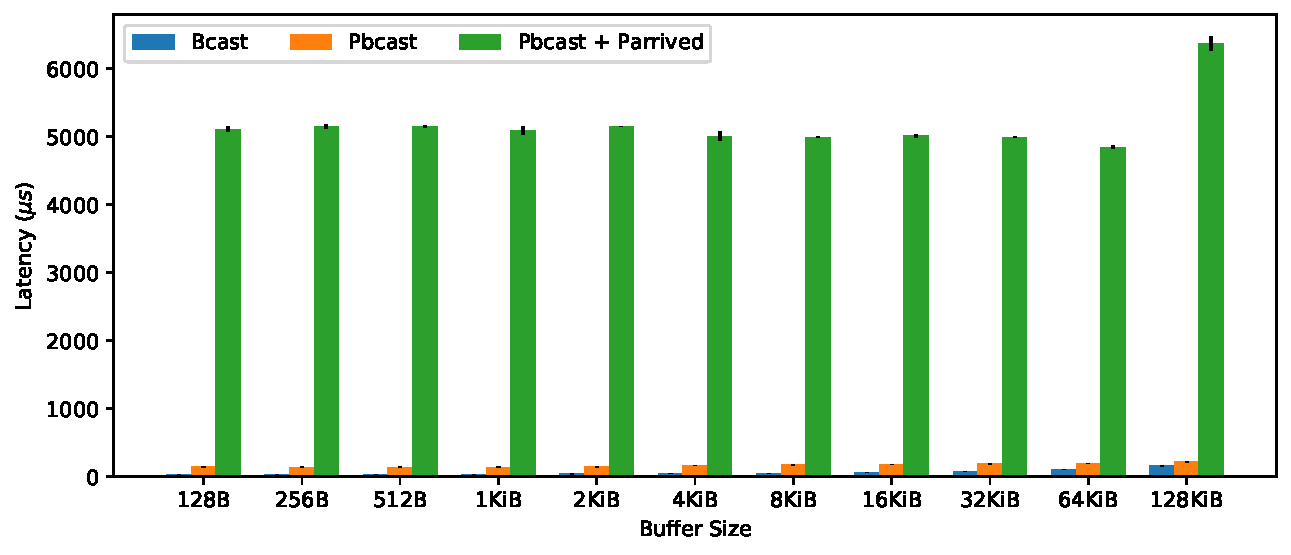
\includegraphics[width=\textwidth]{data-knomial-2-bcast/small_64.pdf}
      \caption{Small}
    \end{subfigure}

    \begin{subfigure}[b]{0.44\textwidth}
      \centering
      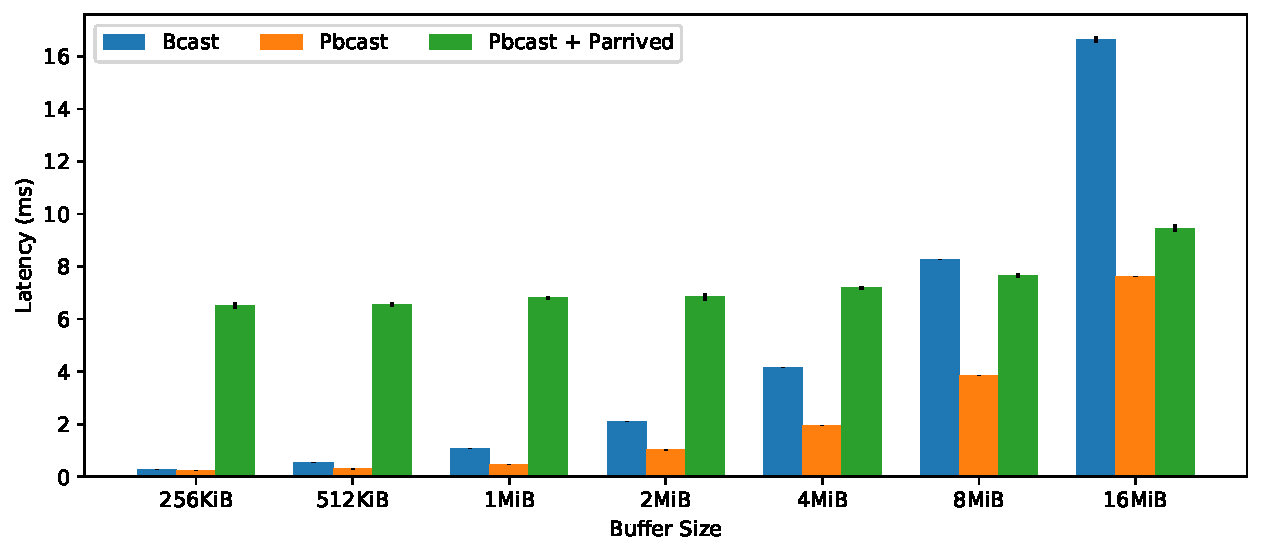
\includegraphics[width=\textwidth]{data-knomial-2-bcast/med_64.pdf}
      \caption{Medium}
    \end{subfigure}
    \hfill

    \begin{subfigure}[b]{0.44\textwidth}
      \centering
      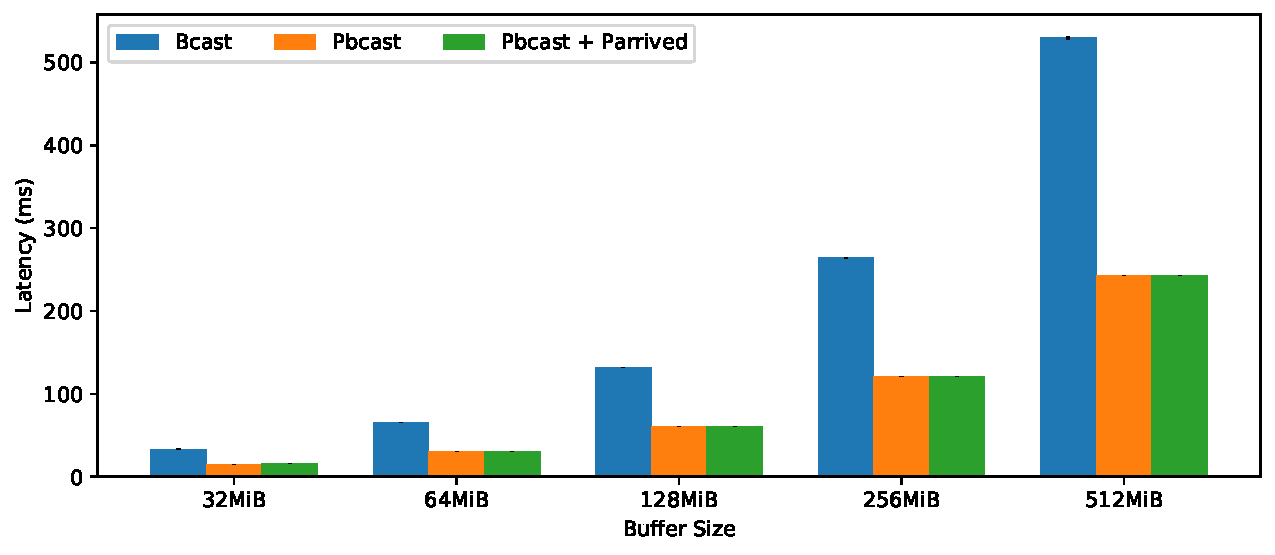
\includegraphics[width=\textwidth]{data-knomial-2-bcast/large_64.pdf}
      \caption{Large}
    \end{subfigure}
    \caption{Comparison of Partitioned and Traditional Broadcast communication
             pattern using the binomial algorithm. Using 64 ranks with 32 threads
             (2048 cores) and $\Delta = 40\mu s$.}
  \end{figure}

  \section{Future Work}
  \subsection{RMA Implementation}

  \subsection{Mapping Graph}
  Currently we have a generic framework which can execute and arbitrary
  partitioned collective.
  To further optimize this we can use some system information:
  \begin{itemize}
    \item \textbf{Slurm Job Information}
    \begin{itemize}
      \item Obtain the nodes in our current allocation
      \item Could even obtain list of inactive node that we could use for
            routing messages on the NC1225.
    \end{itemize}
    \item \texttt{rpcli}
    \begin{itemize}
      \item Obtain the topology of our network
    \end{itemize}
    \item \textbf{Collective Information}
    \begin{itemize}
      \item Typical information like message size, number of partitions, rank
            size, algorithm, etc.
    \end{itemize}
  \end{itemize}

  \noindent
  The goal would be to utilize this information to construct a better
  partitioned collective algorithm

  \begin{figure}[h]
    \centering
    \usetikzlibrary{math}
    \begin{tikzpicture}[scale=.7]
        \tikzmath{ \w = 6; \h = 3; \x = 2; }
        \draw [fill=gray!30,thick] (-\w/2,-\h/2) rectangle (\w/2,\h/2);

        \draw [->,thick] (\w/2, 0) -- (\w/2+\x,0);

        \draw [->,thick] (-\w/2-\x, 0) -- (-\w/2,0);
        \draw [->,thick] (-\w/2-\x, 1) -- (-\w/2,1);
        \draw [->,thick] (-\w/2-\x, -1) -- (-\w/2, -1);

        \node [left] at (-\w/2-\x,0) {\texttt{rpcli}};
        \node [left] at (-\w/2-\x,1) {Slurm Job Information};
        \node [left] at (-\w/2-\x,-1) {Collective Infomation};
        \node [right] at (\w/2+\x, 0) {Optimized Collective Graph};
        \node [align=left,font=\ttfamily] at (0,0) {Mapping Algorithm};
    \end{tikzpicture}
    \caption{High Level Diagram of our Mapping Approach}
  \end{figure}

  \clearpage
  \appendix
  \section{Appendix}
  \label{app:pcomm:bug}
  \subsection{Open MPI's Persistent MPI Partitioned Bug}
  \noindent
  Open MPI's Persistent MPI Partitioned implementation deadlocks (1 in 10 executions),
  if the following conditions are met:
  \begin{itemize}
    \item Partitions \textgreater 16
    \item Iterations \textgreater 2
  \end{itemize}

  \subsubsection{Minimum Bug Creating Example}
  The bug occurs in rank 1 as \texttt{sreq} never completes.
  \singlespacing
  \lstinputlisting[style=CStyle]{pcomm_bug.c}
  \doublespacing

  \clearpage
  \subsection{Bcast - Binomial Algorithm - 8 Ranks}
  \begin{figure}[h]
    \centering
    \begin{subfigure}[b]{0.44\textwidth}
      \centering
      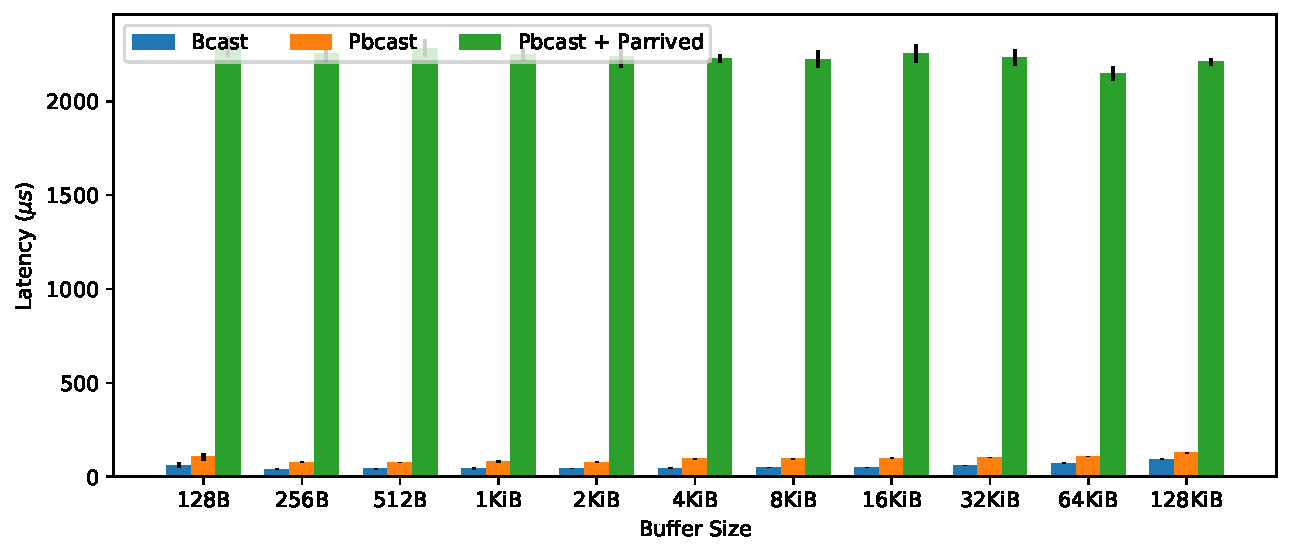
\includegraphics[width=\textwidth]{data-knomial-2-bcast/small.pdf}
      \caption{Small}
    \end{subfigure}

    \begin{subfigure}[b]{0.44\textwidth}
      \centering
      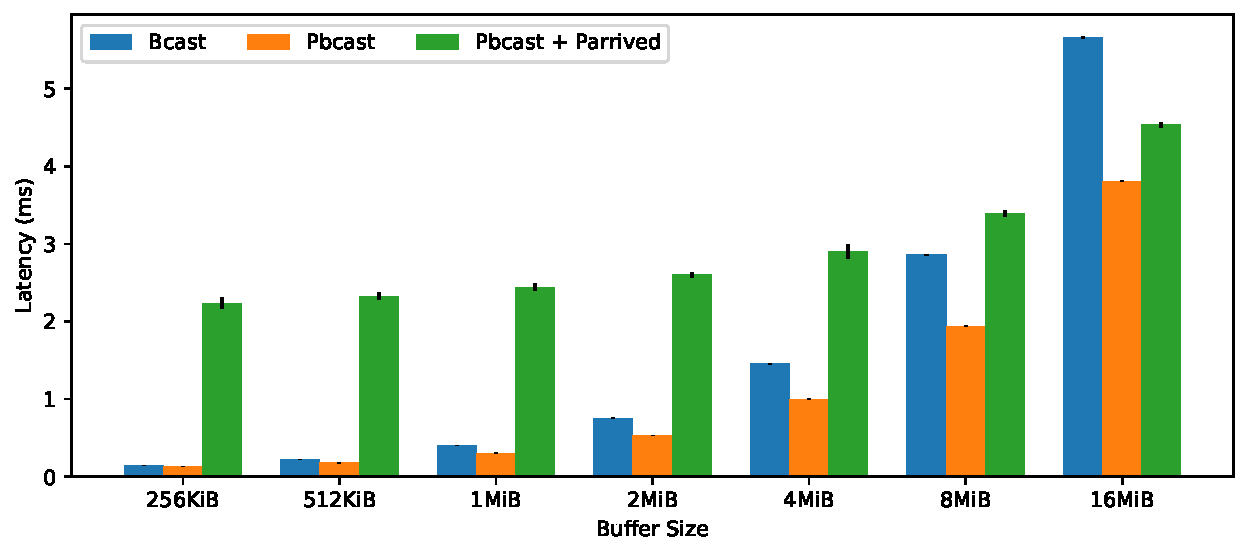
\includegraphics[width=\textwidth]{data-knomial-2-bcast/med.pdf}
      \caption{Medium}
    \end{subfigure}
    \hfill

    \begin{subfigure}[b]{0.44\textwidth}
      \centering
      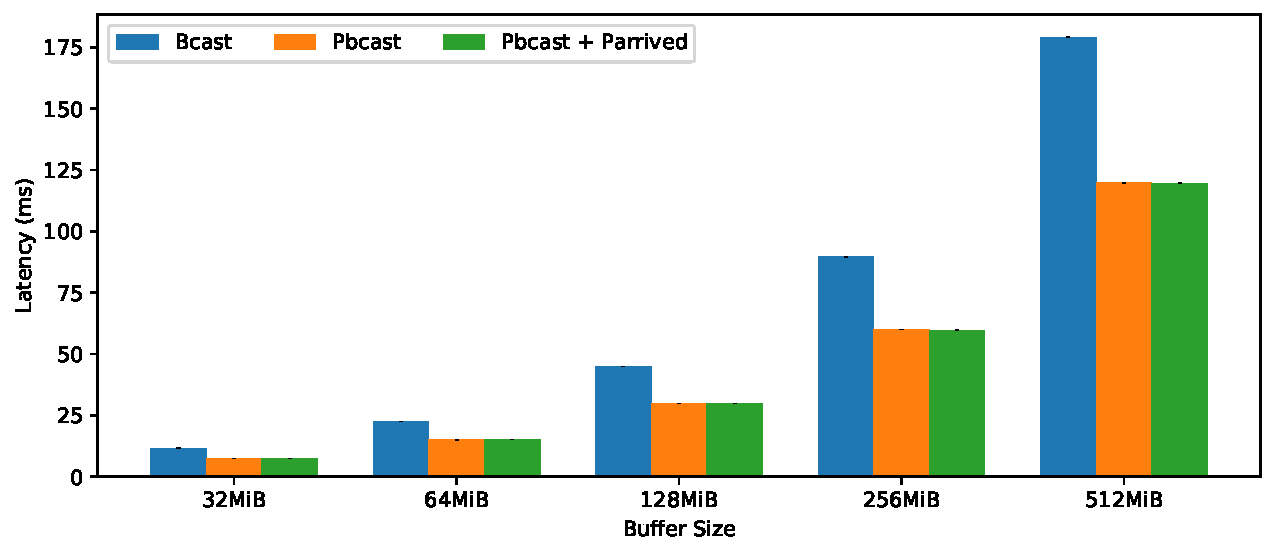
\includegraphics[width=\textwidth]{data-knomial-2-bcast/large.pdf}
      \caption{Large}
    \end{subfigure}
    \caption{Comparison of Partitioned and Traditional Broadcast communication
             pattern using the binomial algorithm. Using 8 ranks with 32 threads
             (256 cores) and $\Delta = 40\mu s$.}
  \end{figure}

  \clearpage
  \addcontentsline{toc}{section}{References}
  \bibliography{cite.bib}
  \bibliographystyle{IEEEtran}
\end{document}
